\documentclass[tikz, border=10pt]{standalone}
\usepackage{amsmath,amssymb}
\usetikzlibrary{shapes.geometric, arrows.meta, positioning, calc, backgrounds, fit}

\begin{document}

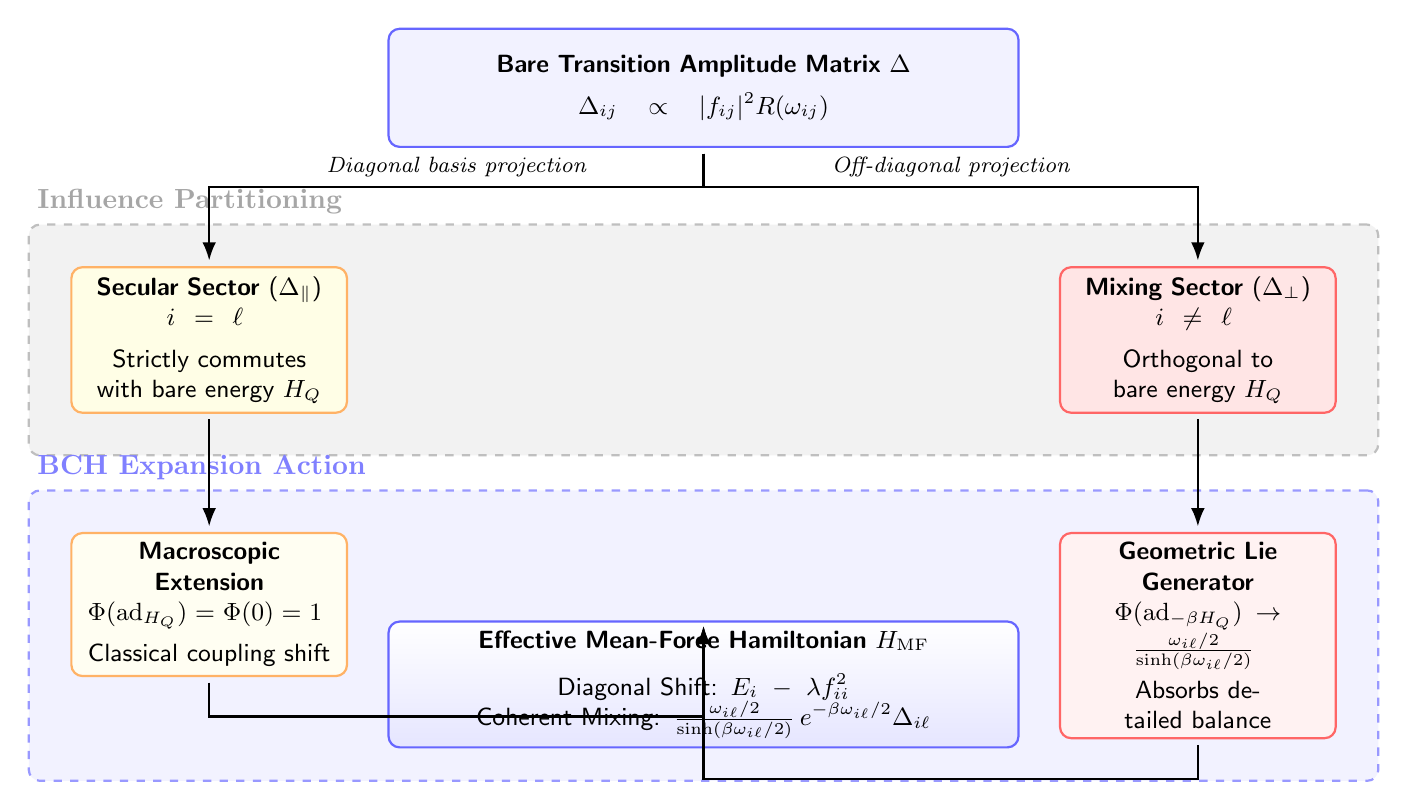
\begin{tikzpicture}[
    node distance=2cm and 2.5cm,
    font=\sffamily\small,
    box/.style={rectangle, draw, rounded corners, minimum width=3.5cm, minimum height=1.5cm, text centered, text width=3.2cm, fill=white, thick},
    titlebox/.style={rectangle, draw=blue!60, fill=blue!5, rounded corners, minimum width=8cm, minimum height=1.5cm, text centered, text width=7.5cm, thick},
    arrow/.style={-Latex, thick, shorten >=2pt, shorten <=2pt},
    dashed_arrow/.style={-Latex, dashed, thick, shorten >=2pt, shorten <=2pt},
    groupbox/.style={rectangle, draw, rounded corners, dashed, inner sep=15pt, fill=gray!5, thick},
    highlight/.style={fill=red!10, draw=red!60},
    glow/.style={fill=yellow!10, draw=orange!60}
]

% Top level input
\node (delta) [titlebox] {\textbf{Bare Transition Amplitude Matrix} $\Delta$ \\ \vspace{4pt} $\Delta_{ij} \propto \lvert f_{ij}\rvert^2 R(\omega_{ij})$ };

% Splitting
\node (parallel) [box, below left=1.5cm and 0.5cm of delta, glow] {\textbf{Secular Sector} ($\Delta_{\parallel}$) \\ $i = \ell$ \vspace{4pt} \\ Strictly commutes with bare energy $H_Q$};
\node (perp) [box, below right=1.5cm and 0.5cm of delta, highlight] {\textbf{Mixing Sector} ($\Delta_{\perp}$) \\ $i \neq \ell$ \vspace{4pt} \\ Orthogonal to bare energy $H_Q$};

% Processes
\node (bch1) [box, below=1.5cm of parallel, fill=yellow!5, draw=orange!60] {\textbf{Macroscopic Extension} \\ $\Phi(\mathrm{ad}_{H_Q}) = \Phi(0) = 1$ \vspace{4pt} \\ Classical coupling shift };
\node (bch2) [box, below=1.5cm of perp, fill=red!5, draw=red!60] {\textbf{Geometric Lie Generator} \\ $\Phi(\mathrm{ad}_{-\beta H_Q}) \to \frac{\omega_{i\ell}/2}{\sinh(\beta\omega_{i\ell}/2)}$ \vspace{4pt} \\ Absorbs detailed balance};

% Output
\node (hmf) [titlebox, bottom color=blue!10, top color=white, below=6cm of delta] {\textbf{Effective Mean-Force Hamiltonian} $H_{\mathrm{MF}}$ \\ \vspace{6pt} 
Diagonal Shift: $E_i - \lambda f_{ii}^2$ \\ 
Coherent Mixing: $\frac{\omega_{i\ell}/2}{\sinh(\beta\omega_{i\ell}/2)} \, e^{-\beta\omega_{i\ell}/2}\Delta_{i\ell}$ };

% Arrows
\draw [arrow] (delta.south) -- ++(0,-0.5) -| (parallel.north) node[pos=0.25, above, font=\footnotesize\itshape] {Diagonal basis projection};
\draw [arrow] (delta.south) -- ++(0,-0.5) -| (perp.north) node[pos=0.25, above, font=\footnotesize\itshape] {Off-diagonal projection};

\draw [arrow] (parallel) -- (bch1);
\draw [arrow] (perp) -- (bch2);

\draw [arrow] (bch1.south) -- ++(0,-0.5) -| (hmf.north);
\draw [arrow] (bch2.south) -- ++(0,-0.5) -| (hmf.north);

% Background labels
\begin{scope}[on background layer]
    \node (bg1) [groupbox, fill=gray!10, draw=gray!50, fit=(parallel) (perp)] {};
    \node [above right, font=\bfseries\color{gray!70}] at (bg1.north west) {Influence Partitioning};
    
    \node (bg2) [groupbox, fill=blue!5, draw=blue!40, fit=(bch1) (bch2)] {};
    \node [above right, font=\bfseries\color{blue!50}] at (bg2.north west) {BCH Expansion Action};
\end{scope}

\end{tikzpicture}

\end{document}
